\documentclass[12pt]{article}

%Packages add more power to LaTeX documents
\usepackage{fullpage} %Otherwise there will be a lot of wasted space at the margins
\usepackage{enumerate} %For the multi-part problem in example #4
\usepackage{amsthm} %For proof environment
\usepackage{amsmath} %For math symbols (like the black square)
\usepackage{graphicx,float,wrapfig} %Including graphics like PDFs and some image formats.
\newcommand\tab[1][1cm]{\hspace*{#1}}

\author{John E. Buckley III}
\title{CSCI 430: Homework 7}


\begin{document}
\maketitle

\section{6.1-1}
Minimum: $2^h$ \newline
Maximum: $2^{h+1}-1$

\section{6.1-3}
If the $n^{th}$ element is the root of the sub-tree then its children will be $\leq$ to it; the same holds for their children as well, all descendants will be $\leq$ the root, thus the root is the largest value.

\section{6.1-4}
The smallest element would reside in one of the leafs, indexed as such: $\frac{n}{2}+1$

\section{6.1-5}
Sorted array A has the following property for any two indexes i<j: $A[i]\leq A[j]$ \newline
Any array is a mini-heap if $A[i]\leq A[left(i)]$ and $A[i]\leq A[right(i)$ where $i<left(i)$ and $i<right(i)$ \newline 
Thus a sorted array is a mini-heap.

\section{6.2-1}
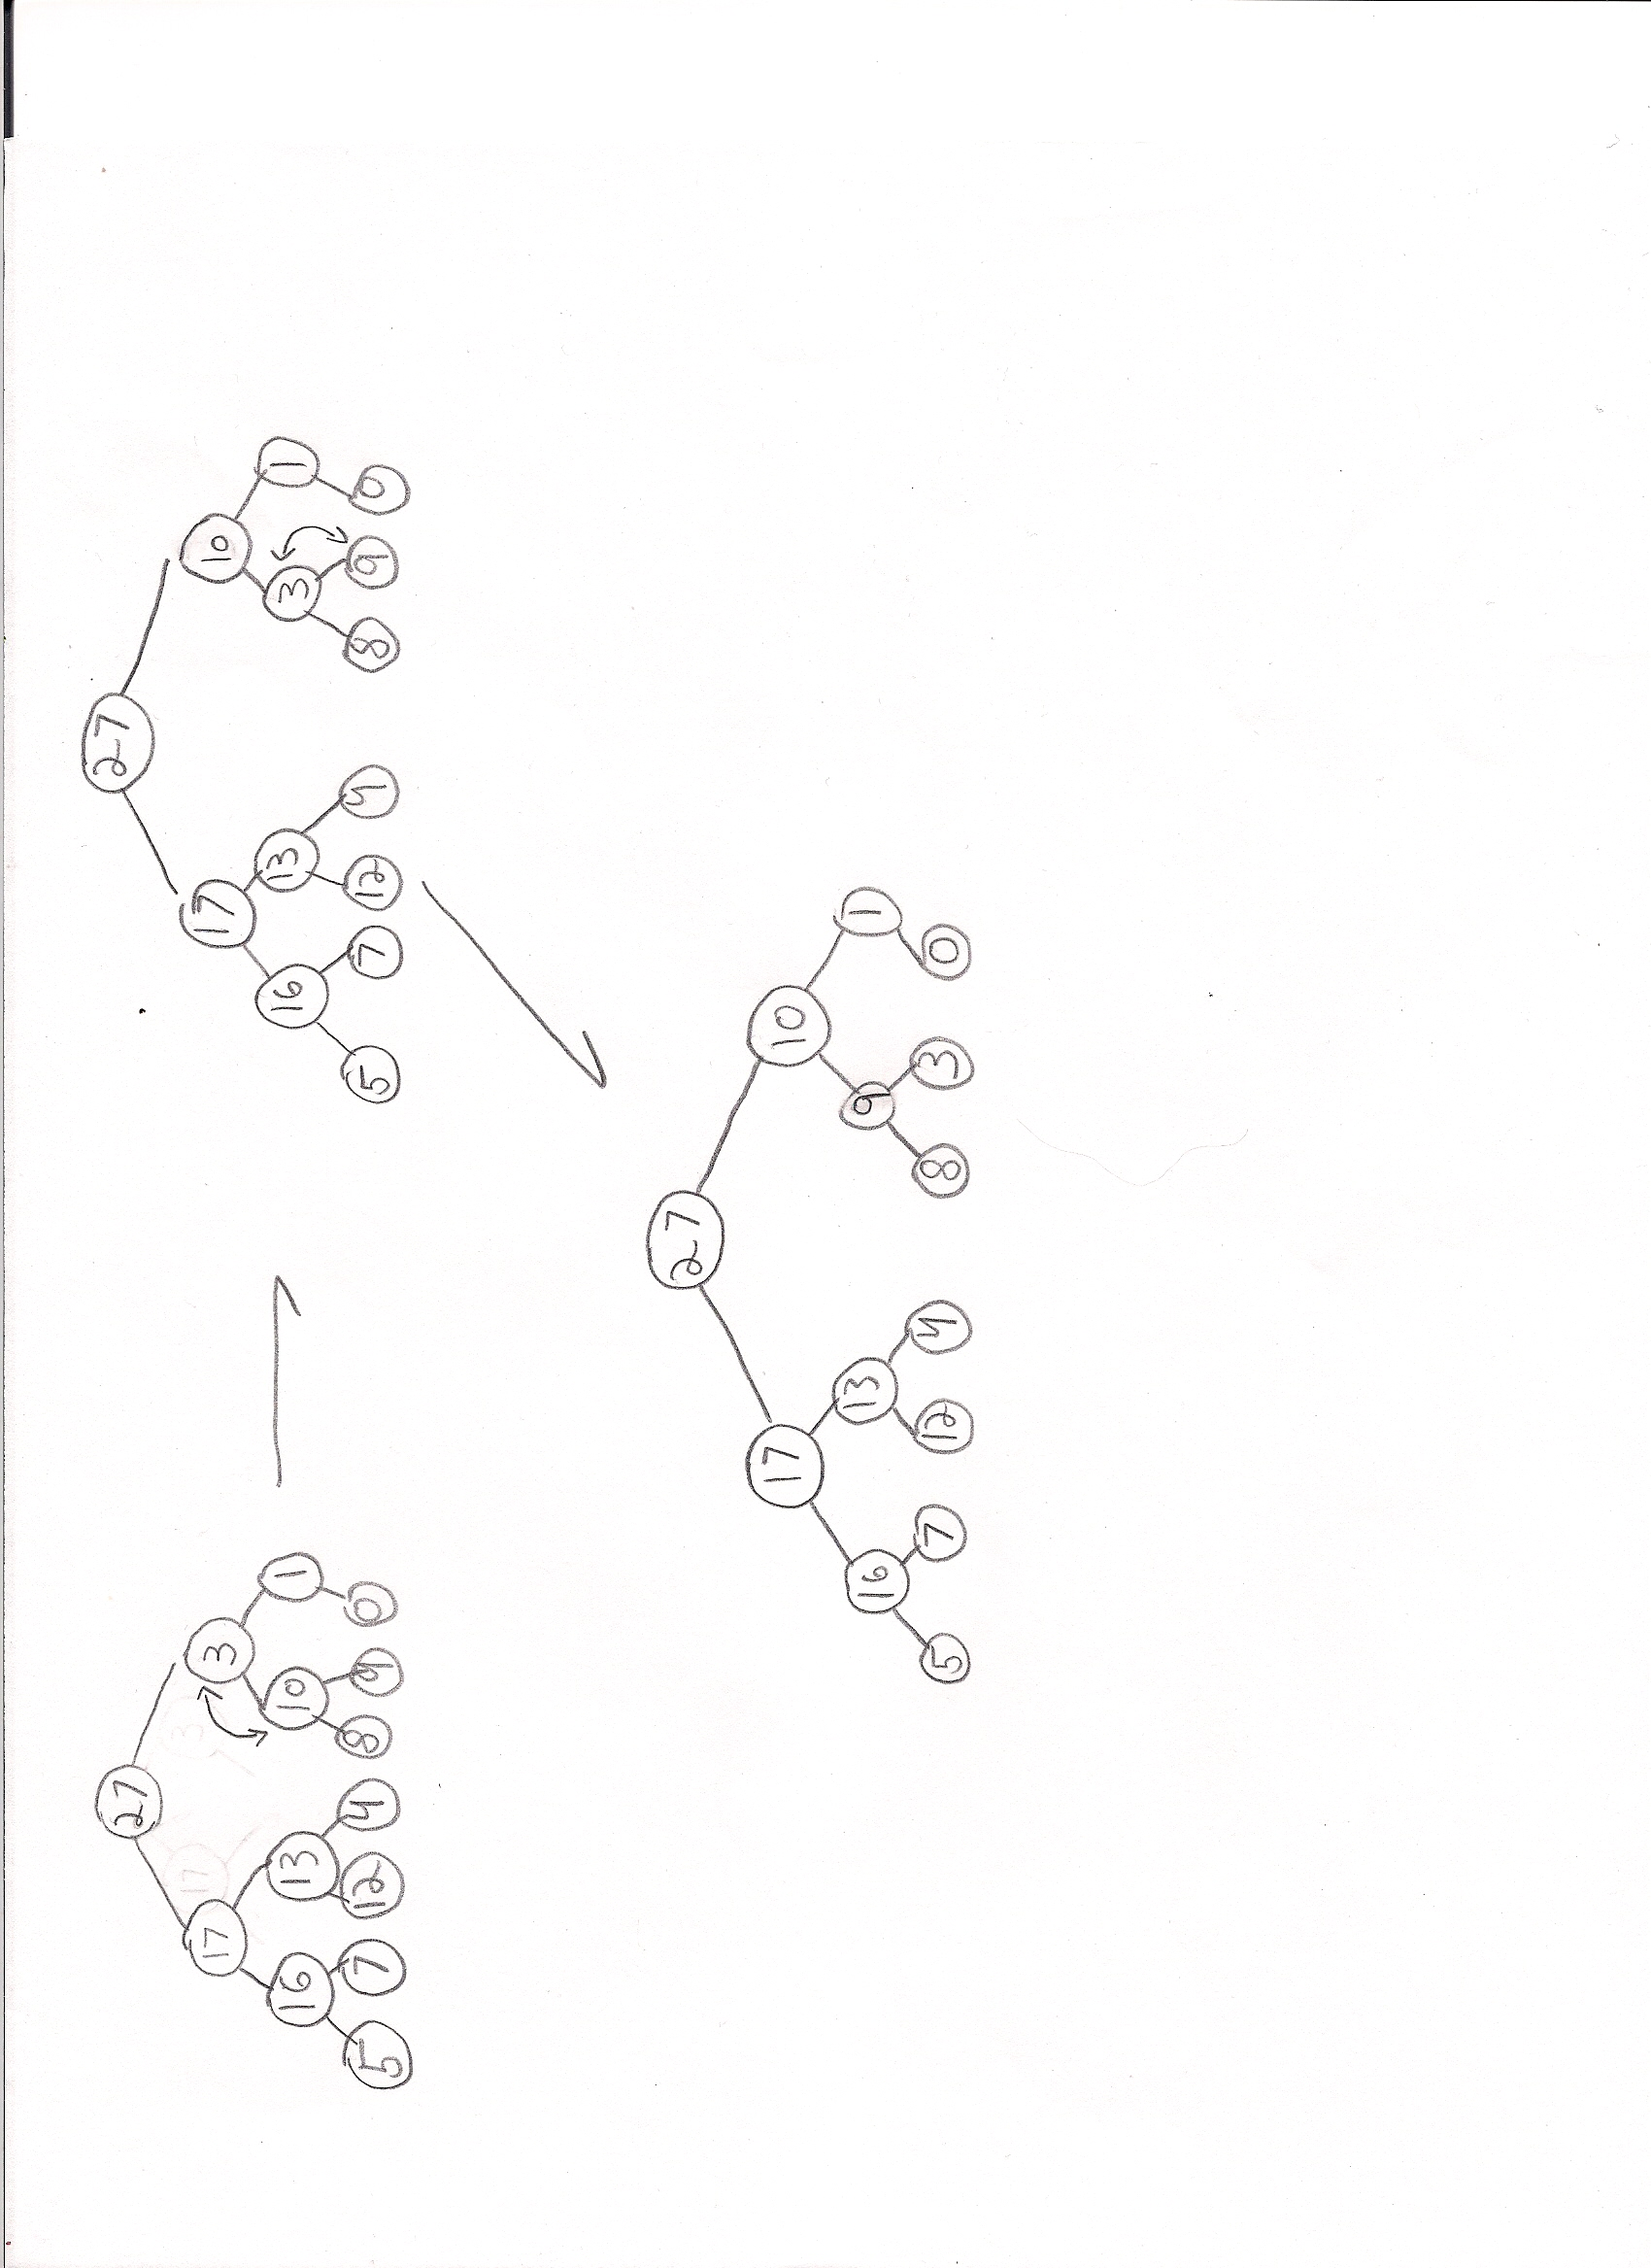
\includegraphics[scale=.5]{blah.jpg}

\section{6.2-3}
There would not be an effect, and since A[i] would be found to be larger than it would simply just return.

\section{6.2-6}
If we were to put the smallest element at the root and was to put the largest elements at the bottom of the left most path in the heap, then MAX-HEAPIFY will be called at every level in the heap in order to move the minimum element to the left most leaf. Thus, since the height of a heap is $lgn$ then the the worst-case running time must be $\Omega(lgn)$

\section{6.3-3}
\textbf{Proof:} by mathematical induction: \newline
\textbf{Base case:} We know that there are $\frac{n}{2}$ leaves in a heap, and nodes of height 0 give us: $\frac{n}{2^{0+1}}$ leaves in an n-element heap. Thus, this holds for the base case of h=0. \newline
\textbf{Inductive step:} Suppose h=k, s.t. there are $\frac{n}{2^{k+1}}$ nodes of height k in an n-element heap. Since heap closely resembles a binary tree, this means that nearly every two nodes with a height of k share a parent at height k+1. This tells us that there are at most $\frac{\frac{n}{2^{k+1}}}{2}$ = $\frac{n}{2^{(k+1)+1}}$ nodes at height k+1. This tells us that this proposition holds for the case when h=k+1. \newline
Therefore, by mathematical induction, there are at most $\frac{n}{2^{h+1}}$ nodes of height h in any n-element heap.

\section{6.4-2}
\textbf{Initialization:} Prior to the first iteration of the loop: i=n, the sub-array A[1...i] is a max-heap, and the sub-array A[i+1...n] is empty. \newline
\textbf{Maintenance:} A[1] is the largest element of A[1...i], A[1] is also smaller than the elements of A[i+1...n]. When we put A[1] in the ith position, then A[i...n] will contain the largest elements in sorted order. Calling MAX-HEAPIFY turns A[1...i-1] into a max-heap. Lastly, decrementing i will set it up for the next iteration. \newline
\textbf{Termination:} The loop terminates when i=1. A[2...n] is sorted and A[1] is the smallest element in the array, thus the array is sorted.


\end{document}